\scanpage{71}
\mspage{3}

sous-groupoïde induit sur une partie \uline{finie} \deleted{\illegible{1}} $I$ de $X_K$, on pourra trouver un nb fini de tels générateurs --- il suffit p.ex. de choisir un \deleted{\unsure{$x$}} $x_0\in I$, et choisir pour tt $x\in I\setminus x_0$ un chemin $l_x$ de $x_0$ \unsure{à|:} $x$, et de plus un syst. \inserted{fini} de générateurs $l_i$ de $\pi_1(X,x_0)$.

\unsure{Il apparaît|Je trouvait} que sous des conditions assez générales (p.ex. si $X$ est une courbe alg. anabélienne) la connaissance de l'opération $u$ sur $\widehat{\Pi}_1(X_K,I)$ (\inserted{pour un} $u\in\Gamma$) \uline{suffit à} déterminer $u$ --- et la question se pose alors de voir comment la connaissance des invariants $g_{l_\alpha}(u)$ \inserted{disons} (pour un syst. générateur de flèches $l_\alpha$ de $\Pi_1(X,\unsure{I})$) permet de retrouver les invariants $g_l(u)$ pour d'autres \inserted{$K$-}schémas $Y\ldots$.

\margin{\figure{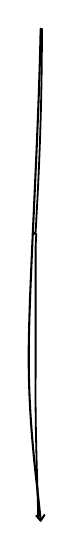
\begin{tikzpicture}[x=.08mm,y=-.08mm,line cap=round,line join=round]
\draw[line width=.65pt] (58,17) .. controls (58,180) and (50,300) .. (48,340)--(43,342)--(49,343)--(48,362) .. controls (48,430) and (48,510) .. (48,565) .. controls (47,655) and (51,738) .. (52,792);
\draw[line width=.75pt] (56,17) .. controls (52,210) and (37,430) .. (37,538) .. controls (37,650) and (50,735) .. (56,798);
\draw[line width=.75pt] (49,790)--(56,798)--(62,789);
\end{tikzpicture}}}

Quand il s'agit du $=$ schéma $X$, et qu'on s'intéresse \unsure{à|:} d'autres chemins $l:x\unsure{\relbar\joinrel\relbar|\longrightarrow}y$ $(x,y\in I)$ que les générateurs choisis $l_\alpha$, la formule (6) donne en principe un moyen de reconstituer les $g_l(u)$ pour tout $l$, puisqu'il permet de retrouver les ${}^u l$, et que ${}^u l$ est multiplicatif en $l$. En termes des $g_l(u)$, \deleted{$\unsure{=}\unsure{f_l(u)}$}, la formule de multiplicativité (6) s'écrit, pour une situation

\margin{\uline{NB} pour le moment, on ne regarde que les $x\in X_K$ qui sont dans $I$, le syst fini de points choisi\unsure{.}}

\diagram{\unsure{\begin{tikzcd}[ampersand replacement=\&,column sep=large]
x\arrow[r,no head,"l'"] \& y\arrow[r,"l^{\deleted{\unsure{''|'}}}"] \& z
\end{tikzcd}}}

\[
(10)\qquad \unsure{g_{ll'}(\deleted{ll'}u)}=g_l(u)\cdot l\bigl(g_{l'}(u)\bigr)
\qquad\text{soit }g_u(ll')=g_u(l)\cdot \unsure{l(g_u l'))|l(g_u(l'))}
\]

\margin{70}
